%\RequirePackage[l2tabu, orthodox]{nag}
\RequirePackage{currfile}
\documentclass[12pt]{beamer}
\graphicspath{{Imagenes/}{../Imagenes/}}
\usepackage[utf8]{inputenc}
\usepackage[spanish]{babel}
\usepackage{standalone}
\usepackage{color}
\usepackage[binary-units=true]{siunitx}
\usepackage{hyperref}
\hypersetup{
  colorlinks=true,
  linkcolor=blue,          % color of internal links (change box color with linkbordercolor)
  citecolor=green,        % color of links to bibliography
  filecolor=magenta,      % color of file links
  urlcolor=cyan,           % color of external links
  linkbordercolor={0 0 1}
}
\usepackage{xcolor, soul}
\usepackage{etoolbox}
\usepackage{amsmath}
\usepackage{amsthm}
\usepackage{physics}
\usepackage{multicol}
\usepackage{graphicx}
\usepackage{bookmark}
\usepackage{longtable}
\usepackage{graphicx}
\usepackage{tikz}
\usepackage[siunitx, RPvoltages]{circuitikz}
\usetikzlibrary{mindmap}
\usetikzlibrary{arrows, patterns, shapes, decorations.markings, decorations.pathmorphing}
\usetikzlibrary{matrix,positioning}
\tikzstyle{every picture}+=[remember picture,baseline]
\usepackage[autostyle,spanish=mexican]{csquotes}
\usepackage{pifont}
\usepackage[font=footnotesize,textfont=it]{caption}
\usepackage{tabulary}
\usepackage{booktabs}
\usepackage[outdir=./]{epstopdf}
%\usepackage{epstopdf}
\usepackage{media9}
\usepackage{multimedia}
\usepackage{bigints}
%\usepackage{enumitem}
\usepackage[os=win]{menukeys}
\usepackage{pifont}
\usepackage{pbox}
\usepackage{alltt}
\usepackage{verbatim}
\usepackage{colortbl}
\usepackage{tcolorbox}
\usepackage{fancyvrb}
\usepackage[sfdefault]{roboto}  %% Option 'sfdefault' only if the base font of the document is to be sans serif
%\usepackage[T1]{fontenc}
\setcounter{secnumdepth}{3}
\setcounter{tocdepth}{3}
\DeclareGraphicsExtensions{.pdf,.png,.jpg}
\renewcommand {\arraystretch}{1.5}
\definecolor{ao}{rgb}{0.0, 0.5, 0.0}
\definecolor{aquamarine}{rgb}{0.5, 1.0, 0.83}
\definecolor{kellygreen}{rgb}{0.3, 0.73, 0.09}
\definecolor{bisque}{rgb}{1.0, 0.89, 0.77}
\definecolor{amber}{rgb}{1.0, 0.75, 0.0}
\definecolor{armygreen}{rgb}{0.29, 0.33, 0.13}
\definecolor{alizarin}{rgb}{0.82, 0.1, 0.26}
\definecolor{cadetblue}{rgb}{0.37, 0.62, 0.63}
\newcommand*{\TitleParbox}[1]{\parbox[c]{6cm}{\raggedright #1}}%
\newcommand{\python}{\texttt{python}}
\newcommand{\textoazul}[1]{\textcolor{blue}{#1}}
\newcommand{\azulfuerte}[1]{\textcolor{blue}{\textbf{#1}}}
\newcommand{\funcionazul}[1]{\textcolor{blue}{\textbf{\texttt{#1}}}}
%\normalfont
\usepackage{ccfonts}% http://ctan.org/pkg/{ccfonts}
\usepackage[T1]{fontenc}% http://ctan.or/pkg/fontenc
\renewcommand{\rmdefault}{cmr}% cmr = Computer Modern Roman
\usefonttheme[onlymath]{serif}
\linespread{1.3}
\newcounter{saveenumi}
\newcommand{\seti}{\setcounter{saveenumi}{\value{enumi}}}
\newcommand{\conti}{\setcounter{enumi}{\value{saveenumi}}}
\newcommand{\tikzmark}[1]{\tikz[remember picture] \node[coordinate] (#1) {#1};}

\usepackage{scalerel}[2016-12-29]
\def\stretchint#1{\vcenter{\hbox{\stretchto[440]{\displaystyle\int}{#1}}}}
\def\scaleint#1{\vcenter{\hbox{\scaleto[3ex]{\displaystyle\int}{#1}}}}
\def\bs{\mkern-12mu}

\newtheorem{teo}{}[section]
\usepackage{blkarray}

%reduce el tamaño de letra de la etiqueta equations
\makeatletter
\def\maketag@@@#1{\hbox{\m@th\normalfont\small#1}}
\makeatother

%se usa para la x en itemize
\newcommand{\xmark}{\text{\ding{55}}}

%\AtBeginDocument{\setlength{\tymin}{1em}}


\definecolor{myblue}{rgb}{.8, .8, 1}

\usepackage{empheq}

\newlength\mytemplen
\newsavebox\mytempbox

\makeatletter
\newcommand\mybluebox{%
    \@ifnextchar[%]
       {\@mybluebox}%
       {\@mybluebox[0pt]}}

\def\@mybluebox[#1]{%
    \@ifnextchar[%]
       {\@@mybluebox[#1]}%
       {\@@mybluebox[#1][0pt]}}

\def\@@mybluebox[#1][#2]#3{
    \sbox\mytempbox{#3}%
    \mytemplen\ht\mytempbox
    \advance\mytemplen #1\relax
    \ht\mytempbox\mytemplen
    \mytemplen\dp\mytempbox
    \advance\mytemplen #2\relax
    \dp\mytempbox\mytemplen
    \colorbox{myblue}{\hspace{1em}\usebox{\mytempbox}\hspace{1em}}}

\makeatother



%Se usa la plantilla Warsaw modificada con spruce
\mode<presentation>
{
  \usetheme{Warsaw}
  \setbeamertemplate{headline}{}
  %\useoutertheme{infolines}
  \usecolortheme{crane}
  \setbeamercovered{invisible}
  

\setbeamertemplate{section in toc}[sections numbered]
\setbeamertemplate{subsection in toc}[subsections numbered]
\setbeamertemplate{subsection in toc}{\leavevmode\leftskip=3.2em\rlap{\hskip-2em\inserttocsectionnumber.\inserttocsubsectionnumber}\inserttocsubsection\par}
\setbeamercolor{section in toc}{fg=blue}
\setbeamercolor{subsection in toc}{fg=blue}
\setbeamerfont{subsection in toc}{size=\small}



\setbeamertemplate{navigation symbols}{}
\setbeamertemplate{caption}[numbered]
% \setbeamercolor{frametitle}{fg=yellow,bg=blue!70!white}
%\setbeamercolor{section in head}{bg=green,fg=white}
%\setbeamercolor{subsection in head/foot}{bg=gray!30,fg=black}
%\setbeamercolor{author in head/foot}{fg=yellow}
%\setbeamercolor{date in head/foot}{fg=blue}

%\mode<presentation>
%{
%  \usetheme{Warsaw}
%  \setbeamertemplate{headline}{}
%  %\useoutertheme{infolines}
%  \useoutertheme{default}
%  \setbeamercovered{invisible}
%  % or whatever (possibly just delete it)
%}
}

\usepackage{courier}
\usepackage{listingsutf8}
\usepackage{listings}
\usepackage{xcolor}
\usepackage{textcomp}
\usepackage{color}
\definecolor{deepblue}{rgb}{0,0,0.5}
\definecolor{brown}{rgb}{0.59, 0.29, 0.0}
\definecolor{OliveGreen}{rgb}{0,0.25,0}
% \usepackage{minted}

\DeclareCaptionFont{white}{\color{white}}
\DeclareCaptionFormat{listing}{\colorbox{gray}{\parbox{0.98\textwidth}{#1#2#3}}}
\captionsetup[lstlisting]{format=listing,labelfont=white,textfont=white}
\renewcommand{\lstlistingname}{Código}


\definecolor{Code}{rgb}{0,0,0}
\definecolor{Keywords}{rgb}{255,0,0}
\definecolor{Strings}{rgb}{255,0,255}
\definecolor{Comments}{rgb}{0,0,255}
\definecolor{Numbers}{rgb}{255,128,0}

\makeatletter

\newif\iffirstchar\firstchartrue
\newif\ifstartedbyadigit
\newif\ifprecededbyequalsign

\newcommand\processletter
{%
  \ifnum\lst@mode=\lst@Pmode%
    \iffirstchar%
        \global\startedbyadigitfalse%
      \fi
      \global\firstcharfalse%
    \fi
}

\newcommand\processdigit
{%
  \ifnum\lst@mode=\lst@Pmode%
      \iffirstchar%
        \global\startedbyadigittrue%
      \fi
      \global\firstcharfalse%
  \fi
}

\lst@AddToHook{OutputOther}%
{%
  \lst@IfLastOtherOneOf{=}
    {\global\precededbyequalsigntrue}
    {}%
}

\lst@AddToHook{Output}%
{%
  \ifprecededbyequalsign%
      \ifstartedbyadigit%
        \def\lst@thestyle{\color{orange}}%
      \fi
    \fi
  \global\firstchartrue%
  \global\startedbyadigitfalse%
  \global\precededbyequalsignfalse%
}

\lstset{ 
language=Python,                % choose the language of the code
basicstyle=\footnotesize\ttfamily,       % the size of the fonts that are used for the code
numbers=left,                   % where to put the line-numbers
numberstyle=\scriptsize,      % the size of the fonts that are used for the line-numbers
stepnumber=1,                   % the step between two line-numbers. If it is 1 each line will be numbered
numbersep=5pt,                  % how far the line-numbers are from the code
backgroundcolor=\color{white},  % choose the background color. You must add \usepackage{color}
showspaces=false,               % show spaces adding particular underscores
showstringspaces=false,         % underline spaces within strings
showtabs=false,                 % show tabs within strings adding particular underscores
frame=single,   		% adds a frame around the code
tabsize=2,  		% sets default tabsize to 2 spaces
captionpos=t,   		% sets the caption-position to bottom
breaklines=true,    	% sets automatic line breaking
breakatwhitespace=false,    % sets if automatic breaks should only happen at whitespace
escapeinside={\#},  % if you want to add a comment within your code
stringstyle =\color{OliveGreen},
%otherkeywords={{as}},             % Add keywords here
keywordstyle = \color{blue},
commentstyle = \color{black},
identifierstyle = \color{black},
literate=%
         {á}{{\'a}}1
         {é}{{\'e}}1
         {í}{{\'i}}1
         {ó}{{\'o}}1
         {ú}{{\'u}}1
%
%keywordstyle=\ttb\color{deepblue}
%fancyvrb = true,
}

\lstdefinestyle{FormattedNumber}{%
    literate={0}{{\textcolor{red}{0}}}{1}%
             {1}{{\textcolor{red}{1}}}{1}%
             {2}{{\textcolor{red}{2}}}{1}%
             {3}{{\textcolor{red}{3}}}{1}%
             {4}{{\textcolor{red}{4}}}{1}%
             {5}{{\textcolor{red}{5}}}{1}%
             {6}{{\textcolor{red}{6}}}{1}%
             {7}{{\textcolor{red}{7}}}{1}%
             {8}{{\textcolor{red}{8}}}{1}%
             {9}{{\textcolor{red}{9}}}{1}%
             {.0}{{\textcolor{red}{.0}}}{2}% Following is to ensure that only periods
             {.1}{{\textcolor{red}{.1}}}{2}% followed by a digit are changed.
             {.2}{{\textcolor{red}{.2}}}{2}%
             {.3}{{\textcolor{red}{.3}}}{2}%
             {.4}{{\textcolor{red}{.4}}}{2}%
             {.5}{{\textcolor{red}{.5}}}{2}%
             {.6}{{\textcolor{red}{.6}}}{2}%
             {.7}{{\textcolor{red}{.7}}}{2}%
             {.8}{{\textcolor{red}{.8}}}{2}%
             {.9}{{\textcolor{red}{.9}}}{2}%
             {\ }{{ }}{1}% handle the space
         ,%
          %mathescape=true
          escapeinside={__}
          }



\makeatletter
%\setbeamercolor{section in foot}{bg=gray!30, fg=black!90!orange}
%\setbeamercolor{subsection in foot}{bg=blue!30!yellow, fg=red}
\setbeamertemplate{footline}
{
  \leavevmode%
  \hbox{%
  \begin{beamercolorbox}[wd=.333333\paperwidth,ht=2.25ex,dp=1ex,center]{author in foot}%
    \usebeamerfont{author in head/foot} \textcolor{red}{\insertsection}
  \end{beamercolorbox}}%
  \begin{beamercolorbox}[wd=.333333\paperwidth,ht=2.25ex,dp=1ex,center]{title in foot}%
    \usebeamerfont{title in head/foot}\insertsubsection
  \end{beamercolorbox}%
  \begin{beamercolorbox}[wd=.333333\paperwidth,ht=2.25ex,dp=1ex,right]{date in head/foot}%
    \usebeamerfont{date in head/foot} \insertshortdate{} \hspace*{2em}
    \insertframenumber{} / \inserttotalframenumber \hspace*{2ex} 
  \end{beamercolorbox}}%
  \vskip0pt%
\makeatother	
\normalfont
\usepackage{ccfonts}% http://ctan.org/pkg/{ccfonts}
\usepackage[T1]{fontenc}% http://ctan.or/pkg/fontenc
\renewcommand{\rmdefault}{cmr}% cmr = Computer Modern Roman
\linespread{1.3}
\title{ED con CDF de orden superior}
\subtitle{Curso de Física Computacional}
\author{M. en C. Gustavo Contreras Mayén}
\date{\today}
\institute{Facultad de Ciencias - UNAM}
\titlegraphic{
\includegraphics[width=1.75cm]{Imagenes/escudo-facultad-ciencias}\hspace*{4.75cm}~%
   
\includegraphics[width=1.75cm]{Imagenes/escudo-unam}
}
\begin{document}
\maketitle
\fontsize{14}{14}\selectfont
\spanishdecimal{.}
\section*{Contenido}
\frame{\tableofcontents[currentsection, hideallsubsections]}
\section{ED con CDF de orden superior}
\frame{\tableofcontents[currentsection, hideothersubsections]}
\subsection{ED de cuarto orden}
\begin{frame}
\frametitle{ED de cuarto orden}
Hemos estado revisando la conexión que hay entre el tema anterior (ED con CDF) con el tema de álgebra matricial.
\end{frame}
\begin{frame}
\frametitle{Dos temas unidos}
Contamos ya con las herramientas conceptuales así como de solución numérica, para abordar un problema que plantea un sistema algebraico donde la expresión matrical, será de gran ayuda.
\end{frame}
\begin{frame}
\frametitle{Dos temas unidos}
Pondremos en marcha la solución de ese sistema, con las herramientas que nos brinda \python{}.
\end{frame}
\begin{frame}
\frametitle{ED de orden superior}
En aras de la brevedad, limitamos nuestra discusión al caso especial en el que las derivadas $y^{\prime}$, así como $y^{\prime \prime \prime}$ no aparecen explícitamente en la ecuación diferencial; es decir, consideramos
\[ y^{(4)} = f(x, y, y^{\prime \prime})\]
\end{frame}
\begin{frame}
\frametitle{Características de la ED}
Suponemos que las dos CDF se presentan en cada extremo del dominio de solución $(a, b)$.
\\
\bigskip
Los problemas de esta tipo se encuentran comúnmente en la teoría de vigas.
\end{frame}
\subsection{Solución de la ED4}
\begin{frame}
\frametitle{Solución de la ED}
Nuevamente, dividimos el dominio de solución en $m$ intervalos de longitud $h$ cada uno.
\\
\bigskip
Sustituyendo las derivadas de $y$ por diferencias finitas en los puntos de malla, obtenemos las ecuaciones de diferencias:
\end{frame}
\begin{frame}
\frametitle{Ecs. en diferencias finitas}
\begin{align}
\begin{aligned}
\dfrac{y_{i-2} - 4 \: y_{i-1} + 6 \: y_{i} - 4 \: y_{i+1} + y_{i+2}}{h^{4}} = \\
= f \left( x_{i} , y_{i}, \dfrac{y_{i-1} - 2 \: y_{i} + y_{i+1}}{h^{2}} \right)
\end{aligned}
\label{eq:ecuacion_08_12}
\end{align}
donde $i = 0, 1, \ldots, m$
\end{frame}
\begin{frame}
\frametitle{Re-escribiendo las ecuaciones}
\fontsize{12}{12}\selectfont
\begin{align}
\begin{aligned}
y_{-2} - 4 \: y_{-1} &+ 6 \: y_{0} - 4 \: y_{1} + y_{2} + \\
&- h^{4} \: f \left( x_{0}, y_{0}, \dfrac{y_{-1} - 2 \: y_{0} + y_{1}}{h^{2}} \right) = 0 \label{eq:ecuacion_08_13a}
\end{aligned} \\
\begin{aligned}
 y_{-1} - 4 \: y_{0} &+ 6 \: y_{1} - 4 \: y_{2} + y_{3} + \\
&- h^{4} \: f \left( x_{1}, y_{1}, \dfrac{y_{0} - 2 \: y_{1} + y_{2}}{h^{2}} \right) = 0 \label{eq:ecuacion_08_13b}
\end{aligned} \\
\begin{aligned}
y_{0} - 4 \: y_{1} &+ 6 \: y_{2} - 4 \: y_{3} + y_{4} + \\
&- h^{4} \: f \left( x_{2}, y_{2}, \dfrac{y_{1} - 2 \: y_{2} + y_{3}}{h^{2}} \right) = 0 \label{eq:ecuacion_08_13c}
\end{aligned} \\
\begin{aligned}
&{} \vdots  \nonumber
\end{aligned}
\end{align}
\end{frame}
\begin{frame}
\frametitle{Re-escribiendo las ecuaciones}
\fontsize{12}{12}\selectfont
\begin{align}
\begin{aligned}
&{} \vdots  \nonumber
\end{aligned} \\
\begin{aligned}
y_{m-3} &- 4 \: y_{m-2} + 6 \: y_{m-1} - 4 \: y_{m} + y_{m+1} + \\
&- h^{4} \: f \left( x_{m-1}, y_{m-1}, \dfrac{y_{m-2} - 2 \: y_{m-1} + y_{m}}{h^{2}} \right) = 0 \label{eq:ecuacion_08_13d}
\end{aligned} \\
\begin{aligned}
y_{m-2} &- 4 \: y_{m-1} + 6 \: y_{m} - 4 \: y_{m+1} + y_{m+2} + \\
&- h^{4} \: f \left( x_{m}, y_{m}, \dfrac{y_{m-1} - 2 \: y_{m} + y_{m+1}}{h^{2}} \right) = 0 \label{eq:ecuacion_08_13e}
\end{aligned}
\end{align}
\end{frame}
\subsection{Condiciones de Frontera}
\begin{frame}
\frametitle{Uso de las condiciones de frontera}
Vemos que hay cuatro incógnitas
\[ y_{2}, y_{1}, y_{m+1}, y_{m+2} \] 
que se encuentran fuera del dominio de la solución y deben eliminarse aplicando las condiciones de frontera.
\\
\bigskip
Para ello, nos apoyamos con la siguiente tabla:
\end{frame}
\begin{frame}
\frametitle{Condiciones de frontera para $\alpha$}
\begin{tabular}{| r | m{8cm} |} \hline
CDF & Expresión equivalente de Dif. Fin. \\ \hline
$y(a) = \alpha$ & $y_{0} = \alpha$ \\ \hline
$y^{\prime}(a) = \alpha$ & $y_{-1} = y_{1} - 2 \: h \: \alpha$ \\ \hline
$y^{\prime \prime}(a) = \alpha$ & $y_{-1} = 2 \: y_{0} - y_{1} + h^{2} \: \alpha$ \\ \hline
$y^{\prime \prime \prime}(a) = \alpha$ & $y_{-2} = 2 \: y_{1} - 2 \: y_{1} + y_{2} - 2 \: h^{3} \: \alpha$ \\ \hline
\end{tabular}
\end{frame}
\begin{frame}
\frametitle{Condiciones de frontera para $\beta$}
\begin{tabular}{| r | m{8cm} |} \hline
CDF & Expresión equivalente de Dif. Fin. \\ \hline
$y(b) = \beta$ & $y_{m} = \beta$ \\ \hline
$y^{\prime}(b) = \beta$ & $y_{m+1} = y_{m-1} - 2 \: h \: \beta$ \\ \hline
$y^{\prime \prime}(b) = \beta$ & $y_{m+1} = 2 \: y_{m} - y_{m-1} + h^{2} \: \beta$ \\ \hline
$y^{\prime \prime \prime}(b) = \beta$ & $y_{m+2} = 2 \: y_{m+1} - 2 \: y_{m-1} + y_{m-2} - 2 \: h^{3} \: \beta$ \\ \hline
\end{tabular}
\end{frame}
\begin{frame}
\frametitle{Sobre las CDF}
Mirando detenidamente, se puede notar que algunas combinaciones de las CDF no funcionarán para eliminar el \enquote{exceso}.
\\
\bigskip
\pause
Una de estas combinaciones es claramente $y(a) = \alpha_{1}$ y $y^{\prime \prime \prime}(a) = \alpha_{2}$.
\\
\bigskip
\pause
La otra condición es $y^{\prime}(a) = \alpha_{1}$ y $y^{\prime \prime}(a) = \alpha_{2}$.
\end{frame}
\begin{frame}
\frametitle{Sobre las CDF}
En el contexto de la teoría de vigas, esto tiene sentido: podemos imponer un desplazamiento $y$ o una fuerza de corte $E \: I \: y^{\prime \prime \prime}$ en un punto, \emph{pero es imposible aplicar ambos simultáneamente}.
\end{frame}
\begin{frame}
\frametitle{Sobre las CDF}
De manera similar, no tiene sentido físico indicar tanto la pendiente $y^{\prime}$ como el momento de flexión $E \: I \: y^{\prime \prime}$ en el mismo punto.	
\end{frame}
\subsection{Ejercicio}
\begin{frame}
\frametitle{Ejercicio}
Una viga uniforme de longitud $L$ y con rigidez a la flexión $E \: I$ está unida en los extremos mediante soportes rígidos.
\\
\bigskip
La viga lleva una carga concentrada $P$ en su punto medio.
\begin{figure}
	\centering
	\includestandalone{Figuras/figura_viga_edos}
\end{figure}
\end{frame}
\begin{frame}
\frametitle{Ejemplo}
\begin{figure}
	\centering
	\includestandalone{Figuras/figura_viga_edos}
\end{figure}
Si utilizamos la simetría y modelamos sólo la mitad izquierda de la viga, resolvemos la siguiente ED con CDF y obtenemos el desplazamiento $v$:
\end{frame}
\subsubsection{ED del problema de la viga}
\begin{frame}
\frametitle{ED del problema de la viga}
\[ E \: I \: \dfrac{d^{4} v}{d x^{4}} = 0 \]
\\
Con las CDF
\[v \vert_{x = 0} = 0, \hspace{1cm} \dfrac{d v}{d x} \bigg\vert_{x = 0} = 0 \]
\[ \dfrac{d v}{d x} \bigg\vert_{x = L/2} = 0, \hspace{1cm} E \: I \: \dfrac{d^{3} v}{d x^{3}} \bigg\vert_{x = L/2} = - \dfrac{P}{2} \]
\end{frame}
\subsubsection{Solución}
\begin{frame}
\frametitle{Solución}
Usaremos el método de diferencias finitas para estimar el desplazamiento y el momento de flexión en el punto medio:
\[ M = - E \: I \dfrac{d^{2} v}{d x^{2}} \]
Los valores exactos de la solución son:
\setbeamercolor{item projected}{bg=red!70!black,fg=white}
\setbeamertemplate{enumerate items}[circle]
\begin{enumerate}[<+->]
\item $v = \dfrac{P \: L^{3}}{192 \: E \: I}$ \\
\item $M = \dfrac{P \: L}{8}$
\end{enumerate}
\end{frame}
\begin{frame}
\frametitle{Solución}
Hacemos el siguiente cambio de variable
\[ \xi = \dfrac{x}{L} \hspace{1cm} y = \dfrac{E \: I}{P \: L^{3}} \: v \]
\pause
entonces, tendremos el siguiente problema:
\[ \dfrac{d^{4} y}{d \xi^{4}} = 0 \]
\\
Con las CDF
\[y \vert_{\xi = 0} = 0, \hspace{1cm} \dfrac{d y}{d \xi} \bigg\vert_{\xi = 0} = 0 \]
\[ \dfrac{d y}{d \xi} \bigg\vert_{\xi = 1/2} = 0, \hspace{1cm} \dfrac{d^{3} y}{d \xi^{3}} \bigg\vert_{\xi = 1/2} = - \dfrac{1}{2} \]  
\end{frame}
\subsubsection{Ecs. en diferencias finitas}
\begin{frame}
\frametitle{Ecs. en diferencias finitas}
Escribimos las ecuaciones (\ref{eq:ecuacion_08_13a}) - (\ref{eq:ecuacion_08_13e}), considerando las CDF, de acuerdo a la tabla anterior, las condiciones en el extremo izquierdo son: $y_{0} = 0$ y $y_{-1} = y_{1}$.
\end{frame}
\begin{frame}
\frametitle{Ecs. en diferencias finitas}
De aquí que las ecs. (\ref{eq:ecuacion_08_13a}) y (\ref{eq:ecuacion_08_13b}) son:
\begin{align}
y =& \; 0 \label{eq:ecuacion_a} \\
-4 \: y_{0} + 7 \: y_{1} - 4 \: y_{2} + y_{3} =& \; 0 \label{eq:ecuacion_b}
\end{align}
\pause
La ec. (\ref{eq:ecuacion_08_13c}) es
\begin{align}
y_{0} - 4 \: y_{1} + 6 \: y_{2} - 4 \: y_{3} + y_{4} = 0 \label{eq:ecuacion_c}
\end{align}
\end{frame}
\begin{frame}
\frametitle{Ecs. en diferencias finitas}
En el extremo derecho, las CDF son equivalentes a $y_{m+1} = y_{m-1}$, junto con
\[ y_{m+2} =  2 \: y_{m+1} + y_{m-2} - 2 \: y_{m-1} + 2 \: h^{3} \: (-1/2) = y_{m-2} - h^{3}  \]
\pause
Al sustituir en las ecuaciones (\ref{eq:ecuacion_08_13d}) y (\ref{eq:ecuacion_08_13e}), llegamos a
\begin{align}
y_{m-3} - 4 \: y_{m-2} + 7 \: y_{m-1} - 4 \: y_{m} =& \; 0 \label{eq:ecuacion_d}\\
2 \: y_{m-2} - 8 \: y_{m-1} + 6 \: y_{m} =& \; h^{3} \label{eq:ecuacion_e}
\end{align}
\end{frame}
\subsubsection{Configuración de la matriz}
\begin{frame}
\frametitle{Configuración de la matriz}
La matriz de coeficientes de las ecs. (\ref{eq:ecuacion_a}) - (\ref{eq:ecuacion_e}) se puede hacer simétrica, al dividir la ec. (\ref{eq:ecuacion_e}) entre 2.
\\
\bigskip
Así obtenemos el siguente sistema algebraico:
\end{frame}
\begin{frame}
\frametitle{Sistema matricial del problema}
\[
\begin{bmatrix}
1 &  0 &  0 &    &   & & \\
0 &  7 & -4 &  1 &   & & \\
0 & -4 &  6 & -4 & 1 & & \\
  & \ddots & \ddots & \ddots & \ddots & \ddots & \\
  &  &  1 & -4 & 6 & -4 & 1 \\
  &  &  & 1 & -4 & 7 & -4 \\
  &  &  &   &  1 & -4 & 3
\end{bmatrix}
\begin{bmatrix}
y_{0} \\
y_{1} \\
y_{2} \\
\vdots \\
y_{m-2} \\
y_{m-1} \\
y_{m}
\end{bmatrix} = 
\begin{bmatrix}
0 \\
0 \\
0 \\
\vdots \\
0 \\
0 \\
0.5 \: h^{3}
\end{bmatrix} \]
\end{frame}
\subsubsection{Uso de python}
\begin{frame}
\frametitle{Usando \texttt{scipy.solve\_banded}}
Ahora nos podemos apoyar con la función \azulfuerte{\texttt{solve\_banded}}, que está incluida en \azulfuerte{\texttt{scipy}}.
\\
\bigskip
Para ello, debemos de construir los vectores columna necesarios, a partir de las codiagonales y  de la diagonal principal.
\end{frame}
\begin{frame}
\frametitle{Construcción de los vectores}
Con la función \azulfuerte{\texttt{diagonales}} se construyen los vectores para el arreglo \textbf{\texttt{cm}} -matriz de coeficientes- que requiere la función \azulfuerte{\texttt{solve\_banded}}:
\end{frame}
\begin{frame}[plain, allowframebreaks, fragile]
\frametitle{Función \texttt{diagonales}}
\begin{lstlisting}[caption=Función que construye las codiagonales, style=FormattedNumber, basicstyle=\linespread{1.1}\ttfamily=\small, columns=fullflexible]
def diagonales(x, h, m):
    d = np.ones(m) * 6.0
    e = np.ones(m) * (-4.0)
    f = np.ones(m)
    c = e.copy()
    g = f.copy()
    b = np.zeros(m)
    
    d[_0_] = 1.0
    d[_1_] = 7.0
    d[-_1_] = 3.0
    d[-_2_] = 7.0
    
    e[_0_] = 0.0
    e[_1_] = 0.0
    
    f[_0_] = 0.0
    f[_1_] = 0.0
    f[_2_] = 0.0
    
    c[_0_] = 0.0
    c[-_1_] = 0.0
    
    g[_0_] = 0.0
    g[-_1_] = 0.0
    g[-_2_] = 0.0
    
    b[-_1_] = 0.5 * h**3
    return f, e, d, c, g, b
\end{lstlisting}
\end{frame}
\begin{frame}[plain, fragile]
\frametitle{Geometría de la viga}
\begin{lstlisting}[caption=Geometría de la viga, style=FormattedNumber, basicstyle=\linespread{1.1}\ttfamily=\small, columns=fullflexible]
 # x en el extremo izquierdo
xInicio = 0.0

# x en el extremo derecho
xFinal = 0.5

# numero de puntos en la malla
m = 20 

h = (xFinal - xInicio)/m

x = np.arange(xInicio, xFinal+h, h)
\end{lstlisting}
\end{frame}
\begin{frame}[plain, fragile]
\frametitle{Uso de las codiagonales}
\begin{lstlisting}[caption=Uso de las codiagonales, style=FormattedNumber, basicstyle=\linespread{1.1}\ttfamily=\small, columns=fullflexible]
f, e, d, c, g, b = diagonales(x, h, m+1)

cm = np.array([f, e, d, c, g])

sol = scipy.linalg.solve_\textunderscore_banded((2, 2), cm, b)
\end{lstlisting}
\end{frame}
\begin{frame}[plain, fragile]
\frametitle{Rutina de impresión}
\begin{lstlisting}[caption=Impresión de los resultados, style=FormattedNumber, basicstyle=\linespread{1.1}\ttfamily=\small, columns=fullflexible]
print('punto \t \t desplazamiento')
print('-'*35)

for i in range(len(sol)):
    print('{:1.3e} \t {:1.5e}'.format(x[i], sol[i]))
\end{lstlisting}
\end{frame}
\subsubsection{Gráfica de la solución}
\begin{frame}
\frametitle{Gráfica de la solución}
\vspace{-1cm}
\begin{figure}
	\centering
	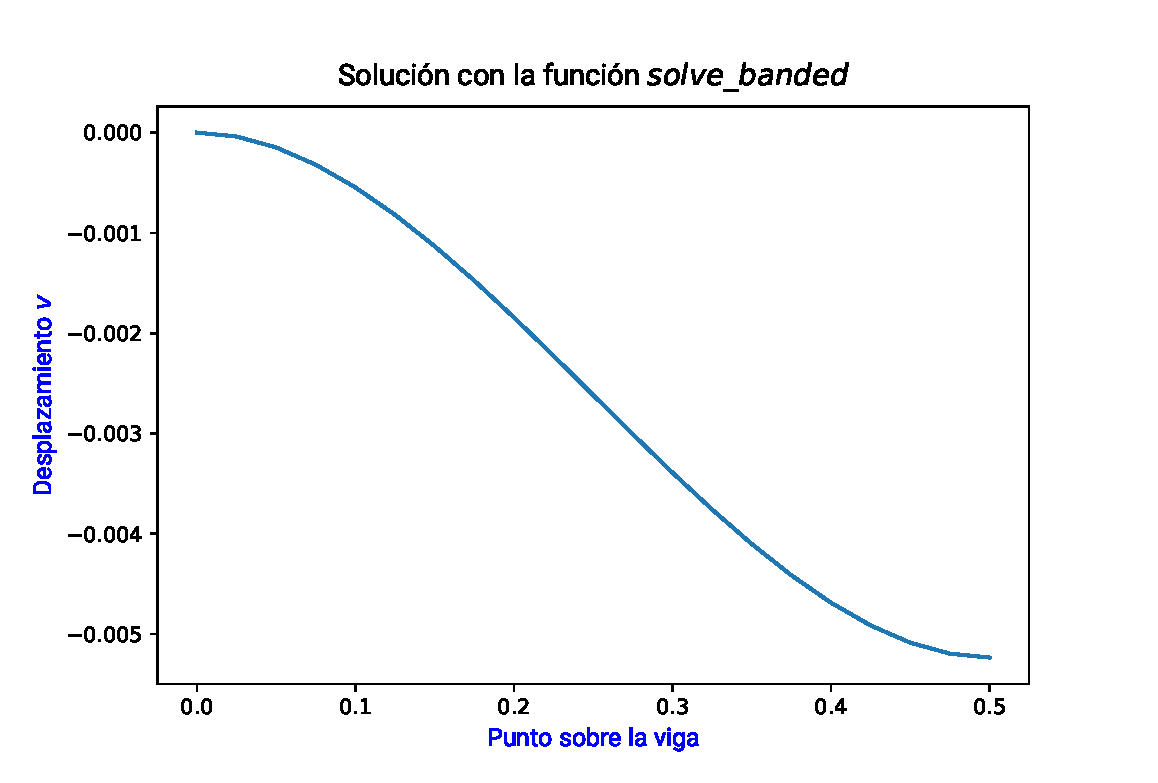
\includegraphics[scale=0.6]{solucion_viga_solve_banded.eps}
\end{figure}
\end{frame}
\subsubsection{Análisis de la solución}
\begin{frame}
\frametitle{Análisis de la solución}
Habiendo ejecutado el programa con $m=20$, tomamos las dos últimas líneas de la solución:
\begin{center}
\begin{tabular}{| c | c| c |} \hline
punto & $x$ & $y$ \\ \hline
$m-1$ & $4.75000e-01$ & $5.19531e-03$ \\ \hline
$m$ & $5.00000e-01$ & $5.23438e-03$ \\ \hline
\end{tabular}
\end{center}
\end{frame}
\begin{frame}
\frametitle{Análisis de la solución}
Por lo tanto, a la mitad de la viga tenemos que:
\[ v \vert_{x=0.5 \: L} = \dfrac{P  \: L^{3}}{E \: I} \: y \bigg\vert_{\xi=0.5} = 5.23438 \times 10^{-3} \; \dfrac{P \: L^{3}}{E \: I} \]
\pause
La solución exacta es:
\[ v \vert_{x=0.5 \: L} = 5.20833 \times 10^{-3} \; \dfrac{P \: L^{3}}{E \: I} \]
\end{frame}
\begin{frame}
\frametitle{Análisis de la solución}
Usamos los valores $m-1$ y $m$ de la solución que recuperamos con el algoritmo:
\fontsize{12}{12}\selectfont
\begin{align*}
\dfrac{d^{2} v}{d x^{2}} \bigg\vert_{x=0.5 \: L} &= \dfrac{P \: L^{3}}{E \: I} \left( \dfrac{1}{L^{2}} \: \dfrac{d^{2} y}{d \xi^{2}} \bigg\vert_{\xi=0.5} \right) \\
&\simeq  \dfrac{P \: L}{E \: I} \: \dfrac{y_{m-1} - 2 y_{m} + y_{m+1}}{h^{2}} \\
&= \dfrac{P \: L}{E \: I} \dfrac{(5.19531 - 2(5.23438) + 5.19531) \times 10^{-3}}{h^{2}} \\
&= -0.125024 \: \dfrac{P \: L}{E \: I}
\end{align*}
\end{frame}
\begin{frame}
\frametitle{Análisis de la solución}
Ya podemos calcular el momento de flexión de la viga:
\begin{align*}
M \big\vert_{x=0.5 \: L} = - E \: I \: \dfrac{d^{2} v}{d x^{2}} \bigg\vert_{\xi=0.5} = 0.125024 \: P \: L
\end{align*}
\pause
La solución exacta es:
\[ M \big\vert_{x=0.5 \: L} = 0.125000 \: P \: L\]
\end{frame}
\begin{frame}[plain]
\frametitle{Gráfica completa de la solución}
%\vspace{-1cm}
\begin{figure}
    \centering
    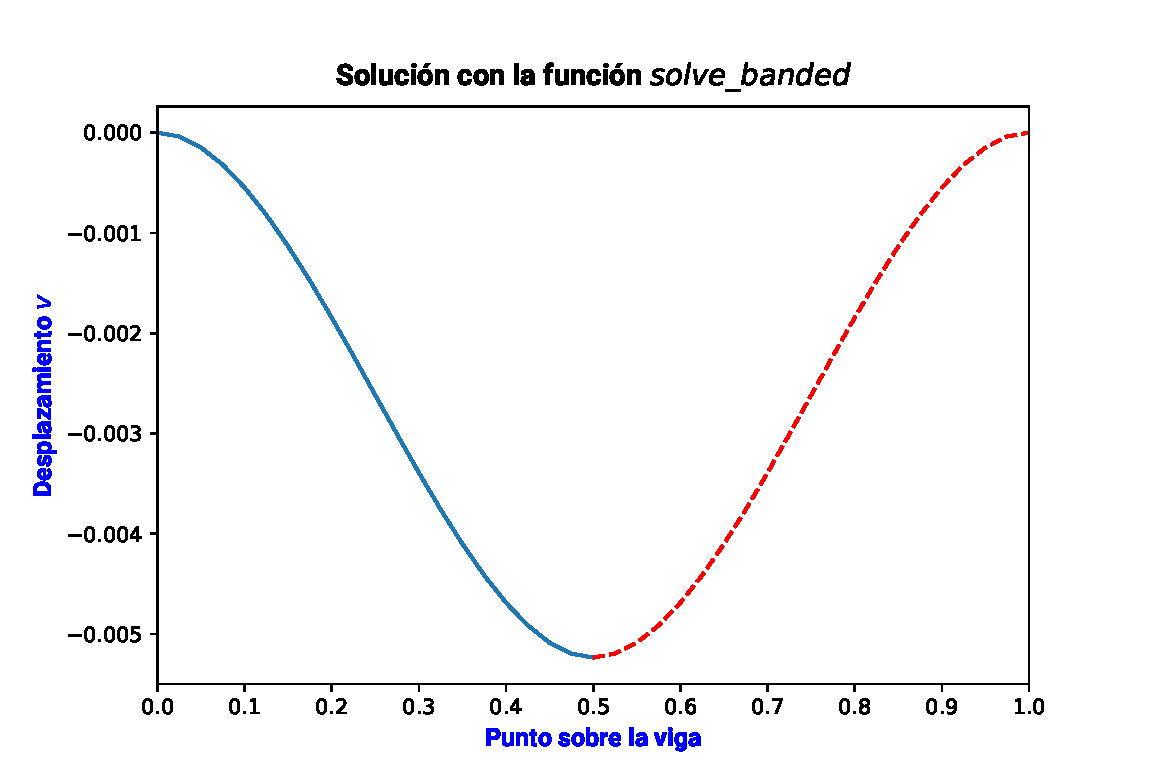
\includegraphics[scale=0.5]{solucion_viga_solve_banded_02.eps}
    \caption{El otro extremo de la viga tiene por simetría, los mismos valores en la solución, sólo invierte el orden de los datos de \funcionazul{sol}.}
\end{figure}
\end{frame}
\section{Funciones para matrices en banda}
\begin{frame}
\frametitle{Uso de funciones para matrices en banda}
 Desarrollamos dos problemas que nos condujeron a un sistema tridiagonal y a otro pentadiagonal.
 \\
 \bigskip
 La elaboración de funciones para factorizar mediante $LU$ y luego resolver la factorización, para cada caso, como vimos es un proceso que sólo funciona en cada problema.
\end{frame}
\begin{frame}
\frametitle{Ventajas con \texttt{scipy}}
Usar la función \azulfuerte{\texttt{solve\_banded}}, no implica complicación mayor (uso de los argumentos), el punto crítico es construir la matriz en banda, mediante el análisis y trabajo propiamente en el cuaderno.
\end{frame}
\begin{frame}
\frametitle{¿Hay más del tema?}
De acuerdo a la orientación que decidan llevar como físicos, encontrarán problemas que les demanden el manejo de soluciones con matrices, lo que se ha revisado, es lo general pero no lo único.
\\
\bigskip
El tema se puede extender más, pero ya enfocado en particular a lo que deban de resolver. Cuentan ya con los elementos básicos para aplicarlo en su formación.
\end{frame}
\subsection{Resolviendo matrices en banda}
% \begin{frame}
% \frametitle{Matrices en banda}
% Muchas matrices grandes tanto en ciencias como en ingeniería son de tal naturaleza, que los elementos de la misma están agrupados (\emph{en banda}).
% \\
% \bigskip
% Lo que significa que sus valores no nulos se encuentran a lo largo de las diagonales de la matriz.
% \end{frame}
% \begin{frame}
% \frametitle{Matrices en banda}
% Se han desarrollado métodos para resolver eficientemente este tipo de matrices.
% \\
% \bigskip
% Las matrices en banda tampoco requieren tanta memoria para almacenar valores intermedios, ya que muchos de las entradas son cero.
% \end{frame}
\begin{frame}[plain]
\frametitle{Considera la siguiente matriz en banda}
\fontsize{12}{12}\selectfont
\begin{align*}
\begin{bmatrix}
1 & -5 & 3 & 0 & 0 & 0 & 0 & 0 \\
3 & 2 & -3 & 5 & 0 & 0 & 0 & 0 \\
0 & -2 & 1 & 5 & 9 & 0 & 0 & 0 \\
0 & 0 & 9 & -1 & 5 & 4 & 0 & 0 \\
0 & 0 & 0 & 0 & 2 & -3 & -2 & 0 \\
0 & 0 & 0 & 0 & 2 & 0 & 1 & -6 \\
0 & 0 & 0 & 0 & 0 & -3 & 2 & 7 \\
0 & 0 & 0 & 0 & 0 & 0 & 9 & 1 
\end{bmatrix}
\end{align*}
\end{frame}
\subsection{Representación de la matriz en banda}
\begin{frame}[plain]
\frametitle{Marcando la diagonal y las codiagonales}
\begin{figure}
    \centering
    \includestandalone[scale=0.8]{Figuras/matriz_marcada_04}    
\end{figure}
\end{frame}
\subsection{Arreglo de las codiagonales}
\begin{frame}
\frametitle{Arreglo de las codiagonales}
\begin{figure}
    \centering
    \includestandalone[scale=0.8]{Figuras/matriz_marcada_05}    
\end{figure}
\begin{itemize}
\item Las codiagonales superiores tienen ceros a la izquierda.
\item Las codiagonales inferiores tienen ceros al final.
\end{itemize}
\end{frame}
\begin{frame}
\frametitle{Nueva representación de la matriz}
La matriz en banda se puede representar por una matriz no cuadrada del tipo
\\
\bigskip
\pause
\[
\begin{blockarray}{ccccccccc}
\begin{block}{c(cccccccc)}
g & 0 & 0 & 3 & 5 & 9 & 4 & -2 & -6 \\
c & 0 & -5 & -3 & 5 & 5 & -3 & 1 & 7 \\
d & 1 & 2 & 1 & -1 & 2 & 0 & 2 & 1 \\
f & 3 & -2 & 9 & 0 & 2 & -3 & 9 & 0 \\
\end{block}
\end{blockarray}
 \]
\end{frame}
\subsection{Función scipy.linalg.solve\_banded()}
\begin{frame}[fragile]
\frametitle{Resolviendo matrices en banda}
Para resolver un sistema de ecuaciones con una matriz en banda, usaremos la función \funcionazul{scipy.linalg.solve\_banded()}.
\\
\bigskip
\pause
La sintaxis para esta función es la siguiente
\begin{alltt}
\funcionazul{solve\_banded((l,u), cm, rhs)}
\end{alltt}
\end{frame}
\begin{frame}[fragile]
\frametitle{Resolviendo matrices en banda}
\begin{alltt}
\funcionazul{solve\_banded((l,u), cm, rhs)}
\end{alltt}
Donde:
\begin{itemize}[<+->]
\item \azulfuerte{\texttt{(l, u)}} es una tupla, donde $l$ es el número de codiagonales inferiores no nulas, y $u$ es el número de codiagonales superiores no nulas.
\item \azulfuerte{\texttt{cm}} es la matriz en banda de coeficientes.
\item \azulfuerte{\texttt{rhs}} es el vector de constantes del lado derecho.
\end{itemize}
\end{frame}
\begin{frame}[plain]
\frametitle{Ejercicio 1 - Matriz en banda}
Resuelve el siguiente sistema algebraico
\begin{align*}
\begin{bmatrix}
1 & -5 & 3 & 0 & 0 & 0 & 0 & 0 \\
3 & 2 & -3 & 5 & 0 & 0 & 0 & 0 \\
0 & -2 & 1 & 5 & 9 & 0 & 0 & 0 \\
0 & 0 & 9 & -1 & 5 & 4 & 0 & 0 \\
0 & 0 & 0 & 0 & 2 & -3 & -2 & 0 \\
0 & 0 & 0 & 0 & 2 & 0 & 1 & -6 \\
0 & 0 & 0 & 0 & 0 & -3 & 2 & 7 \\
0 & 0 & 0 & 0 & 0 & 0 & 9 & 1 
\end{bmatrix}
\begin{bmatrix}
x_{1} \\
x_{2} \\
x_{3} \\
x_{4} \\
x_{5} \\
x_{6} \\
x_{7} \\
x_{8}
\end{bmatrix}
=
\begin{bmatrix}
5 \\
3 \\
-3 \\
2 \\
0 \\
7 \\
8 \\
1
\end{bmatrix}
\end{align*}
\end{frame}
\begin{frame}
\frametitle{Solución al sistema}
\begin{align*}
x_{1} &= 200.639937 \\
x_{2} &= -25.491352 \\
x_{3} &= -107.698899 \\
x_{4} &= -174.206761 \\
x_{5} &= 102.750000 \\
x_{6} &= 70.833333 \\
x_{7} &= -3.500000 \\
x_{8} &= 32.500000
\end{align*}
\end{frame}
\begin{frame}[fragile, plain]
\frametitle{Orden de los vectores renglón}
Hay que tener cuidado al momento de organizar los vectores renglón que conformarán el arreglo \funcionazul{cm}:
\begin{lstlisting}[caption=Definición de los vectores renglón, style=FormattedNumber, basicstyle=\linespread{1.1}\ttfamily=\small, columns=fullflexible]
g = [0. ,0, 3, 5, 9, 4, -2, -6]
c = [0., -5, -3, 5, 5, -3, 1, 7]
d = [1., 2, 1, -1, 2, 0, 2, 1]
e = [3., -2, 9, 0, 2, -3, 9, 0]

b = np.array([5., 3, -3, 2, 0, 7, 8, 1])

cm = np.array([g, c, d, e])
\end{lstlisting}
\end{frame}
\begin{frame}
\frametitle{Solución al problema}
Una vez que definimos el orden de los vectores renglón, ya podemos usar la función \funcionazul{solve\_banded} para encontrar la solución.
\end{frame}
\begin{frame}
\frametitle{Uso de una librería de formato}
Cuando tenemos que presentar en la terminal un conjunto de datos, en ocasiones invertimos más tiempo en ajustar el formato de salida: dejando espacios, tabuladores, etc.   
\end{frame}
\begin{frame}
\frametitle{La librería Texttable}
Usaremos la librería \funcionazul{Texttable} para ahorrar tiempo y dejar una salida en la terminal mucho más amigable.
\end{frame}
\begin{frame}[fragile]
\frametitle{La librería Texttable}
\textbf{Primer paso:} Abre una terminal de comandos, en Linux con la combinación \keys{Control} + \keys{Mayus} + \keys{T}
\\
\bigskip
Escribe la instrucción:
\begin{verbatim}    
pip install texttable
\end{verbatim}
\pause
Esto nos dejará la librería para su uso global.
\end{frame}
\begin{frame}
\frametitle{En tu código}
\textbf{Segundo paso: } Haremos una modificación en el código para mostrar los resultados en la terminal con la nueva librería \funcionazul{Texttable}.
\end{frame}
\begin{frame}[fragile]
\frametitle{Código para elaborar la tabla}
En el apartado de encabezados, donde se importan las librerías:
\begin{lstlisting}[caption=Importando la librería Texttable, style=FormattedNumber, basicstyle=\linespread{1.1}\ttfamily=\small, columns=fullflexible]
import texttable as tt
\end{lstlisting}
\end{frame}
\begin{frame}[fragile, plain]
\frametitle{Código para elaborar la tabla}
\begin{lstlisting}[caption=Creando el objeto y definiendo propiedades, style=FormattedNumber, basicstyle=\linespread{1.1}\ttfamily=\small, columns=fullflexible]
tabla = tt.Texttable()

x = [[]]

for i in range(8):
    x.append(['x' + str(i+1), sol[i]])

tabla.add_\textunderscore_rows(x)
tabla.header(['x', 'Solucion'])
tabla.set_\textunderscore_cols_\textunderscore_align(["c", "l"])
print(tabla.draw())
\end{lstlisting}    
\end{frame}
\begin{frame}[plain, fragile]
\frametitle{Salida en la terminal}
\fontsize{12}{12}\selectfont
\begin{figure}
\centering
\begin{BVerbatim}
+----+----------+
| x  | Solución |
+====+==========+
| x1 | 200.640  |
+----+----------+
| x2 | -25.491  |
+----+----------+
| x3 | -107.699 |
+----+----------+
| .. |   ...    |
+----+----------+
| x7 | -3.500   |
+----+----------+
| x8 | 32.500   |
+----+----------+
\end{BVerbatim}
\end{figure}
\end{frame}
\begin{frame}
\frametitle{Tabla con formato}
Como podrás ver, la tabla que se muesta en la terminal ajusta los contenidos a partir de las propiedades de alineación (\funcionazul{['c', 'l']}), ajusta hacia el centro y a la izquierda.
\\
\bigskip
En la documentación de la librería podrás encontrar más referencias para ajustar tu salida en la terminal con una presentación más profesional.
\end{frame}
% \begin{frame}
% \frametitle{Ejercicio 2 - Matriz tridiagonal simétrica}
% Usando la función \azulfuerte{\texttt{solve\_banded()}}, resuelve el sistema $\mathbf{A \: x} = \mathbf{b}$ (que ya habíamos trabajado), donde
% \begin{equation*} 
% \mathbf{A} =  \begin{bmatrix}
% 2 & -1 & 0 & 0 & 0 \\
% -1 & 2 & -1 & 0 & 0 \\
% 0 & -1 & 2 & -1 & 0 \\
% 0 & 0 & -1 & 2 & -1 \\
% 0 & 0 & 0 & -1 & 2
% \end{bmatrix}
% \hspace{1cm}
% \mathbf{b} =
% \begin{bmatrix}
% 5 \\
% -5 \\
% 4 \\
% -5 \\
% 5
% \end{bmatrix}
% \end{equation*}
% \end{frame}
% \begin{frame}
% \frametitle{Solución al sistema tridiagonal simétrico}
% Cuando usamos las funciones \azulfuerte{\texttt{LUdescomp3}} y \azulfuerte{\texttt{LUsoluc3}} para este sistema tridiagonal simétrico, la solución obtenida es:
% \\
% \bigskip
% \pause
% \[x = [ 2. \; -1. \;\; 1. \; -1. \;\;  2.] \]
% Que debe de ser la misma solución con la función \azulfuerte{\texttt{solve\_banded()}}
% \end{frame}
\end{document}